\errorcontextlines=9999
\documentclass[
   aspectratio=169, % default is 43
   10pt, % font size, default is 11pt
   % nosectionframes,
   uniqueslidenumber,
   handout,
   professionalfonts
]{beamer}

\usepackage[T1]{fontenc}
\usepackage[utf8]{inputenc}
\usepackage[sfdefault]{FiraSans}

\usepackage{stmaryrd}
\usepackage[vvarbb]{notomath}
\usepackage{FiraMono}
\usepackage{tikz,forest}
\usepackage{fontawesome}
\usepackage{csquotes}
\usepackage{relsize}
\usepackage{simplebnf}
\usepackage{../abstract-interpretation-ltx/absint}
\makeatletter
\def\absint@reflab#1#2{#2}% we do not need labels here
\usetikzlibrary{arrows.meta,decorations.pathmorphing,fit,decorations.pathreplacing,backgrounds,matrix}
\pgfdeclarelayer{foreground}
\usepackage[glows]{tikzpingus}
\pgfsetlayers{very-background,background,main,middle,foreground}
\def\sbseries{\fontseries{sb}\selectfont}
\def\textsb#1{{\sbseries#1}}
\tikzset{bottom note/.style={font=\scriptsize,scale=.8,color=gray}}
\usepackage{../slide-template-uulm/fancybeamer} % use the fancy beamer package
\usepackage{../slide-template-uulm/fancyuulm}
\setpaths{{../slide-template-uulm/}{../slide-template-uulm/logos/}{../slide-template-uulm/empty-slides/}{../xlistings/}}

\usepackage{../code-animation/code-animation}
\usepackage[fakeminted,print]{../xlistings/xlistings}
\usepackage{multirow}
\xlstsetmintedstyle{plain}
\LoadLanguages{R,Java}
\lstcolorlet{keywordA}{black!70!red}%
\lstcolorlet{keywordB}{black!70!red}%
\lstcolorlet{keywordC}{black!70!red}%
\lstcolorlet{numbers}{black!70!yellow}%
\def\absintstyle#1{#1}

% bib
\usepackage[style=alphabetic,backend=biber]{biblatex}
\addbibresource{./references.bib}

\title{Static Analysis in the Real World}
\subtitle[SQA]{Software Quality Assurance - Static Code Analysis, III}
\author[F. Sihler]{Florian Sihler}
\date{\today} % use a particular date here if needed

\fancylogos{sp,uulm} % define logos that are spread evenly across the bottom of the title slide

\usepackage{../beamer-latex-pdfpc-notes}

\begin{document}

\maketitle[titleimage/title][40]

\mode
<handout>

\begin{frame}{Outline}
% \begin{multicols}{2}
\tableofcontents[hideallsubsections]
% \end{multicols}
\end{frame}

\mode
<all>

\section{Introduction}

\newsavebox\abstractionbox
\begin{lrbox}{\abstractionbox}
\begin{tikzpicture}[line cap=round]
   \pgfonlayer{foreground}
   \draw[Kite-Kite,very thick] (0,3.5) node[below right,yshift=1mm] {\(x(t)\)} |- (8,0) node[above left] {\(t\)}; % time vs. x at tat time
   \endpgfonlayer
   \colorlet{@}{gray}
   \draw[very thick,@] (0,1) plot [smooth] coordinates {(0,1) (1,2) (2,1) (3,2) (4,1) (5,2) (6,1) (7,2) (8,1)}; % x(t)
   \draw[very thick,@] (0,0) plot [smooth] coordinates {(0,0) (1,1) (2,2) (3,2) (4,2.5) (5,2.5) (6,.5) (7,.6) (8,.6)}; % x(t)
   \draw[very thick,@] (0,1.5) plot [smooth] coordinates {(0,1.5) (1,2) (2,2.5) (3,2) (4,2) (5,2.5) (6,2.5) (7,2) (8,2.5)}; % x(t)
      \foreach \i in {0,...,5} {
         \pgfmathsetmacro{\randA}{rnd*0.33}
         \pgfmathsetmacro{\randB}{rand*0.5}
         \pgfmathsetmacro{\randC}{rand*0.4}
         \draw[gray] (0,1.5+\randA) plot [smooth] coordinates {(0,1.5+\randA) (1,2-\randB) (2,2.5-\randA) (3,2-\randB) (4,2+\randA) (5,2.5) (6,2.5+\randA) (7,2-\randA) (8,2.5+\randB)} node[inner sep=0pt] (a-\i) {};
         \draw[gray] (0,0+\randA) plot [smooth] coordinates {(0,0+\randA) (1,1-\randB) (2,2-\randB) (3,2+\randC) (4,2.5-\randA) (5,2.5-\randB) (6,.5+\randC) (7,.6+\randB) (8,.6+\randC)} node[inner sep=0pt] (b-\i) {};
         \draw[gray] (0,1+\randB) plot [smooth] coordinates {(0,1-\randC) (1,2-\randB) (2,1+\randB) (3,2-\randA) (4,1+\randA) (5,2-\randB) (6,1) (7,2-\randC) (8,1+\randA)} node[inner sep=0pt] (c-\i) {};
      }
   % fit to all nodes to get the bounding box
   \node[fit=(a-0) (a-1) (a-2) (a-3) (a-4) (a-5) (b-0) (b-1) (b-2) (b-3) (b-4) (b-5) (c-0) (c-1) (c-2) (c-3) (c-4) (c-5),inner sep=0pt] (big-ghost) {~};
      % \draw[decorate,thick,decoration={brace,amplitude=5pt,raise=2pt},gray] (big-ghost.north east) -- (big-ghost.south east);
   \pgfonlayer{background}
   \pgfinterruptboundingbox
   \fill[red,opacity=.175,even odd rule] plot [smooth] coordinates {(0,0) (1,0.4) (2,0.5) (3,1) (4,.8) (5,1) (6,.1) (7,0.2) (8.03,.2) (8.03,3) (7,2.8) (6,3) (5,2.95) (4,2.85) (3,2.75) (2,2.65) (1,2.5) (0,2) } -- cycle (6,1.85) circle[radius=4mm]; 
   \endpgfinterruptboundingbox
      \node (@b1) at (6,1.85) {\small\faBug};
      \node (@b2) at (3,.35) {\small\faBug};
      \node (@b3) at (7,2.5) {\small\faBug};
      \node[above left=-1mm,green] at(@b2.south east) {\scriptsize\faCheck};
      \node[above left=-1mm,green] at(@b1.south east) {\scriptsize\faCheck};
      \node[above left=-1mm,yshift=1pt,orange] at(@b3.south east) {\scriptsize\faQuestion};
   \endpgfonlayer
   \path[use as bounding box] (0,0) rectangle (8,3.5);
\end{tikzpicture}
\end{lrbox}

\begin{frame}{What we have\ldots}
\frametitle<-8>{\strut What we have\ldots}%
\frametitle<9->{\strut\textcolor{gray}{What we have\ldots~}Theory}%
\pgfmathsetseed{42}%
\begin{uncoverenv}<2->  
\begin{tikzpicture}[baseline={([yshift=-.5ex]current bounding box.center)},line cap=round]
   \tikzset{@/.style={opacity=1}}
   \def\scaler{1}
   \only<4->{\def\scaler{0.5}\tikzset{@/.style={opacity=.5,scale=.5,every node/.style={transform shape}}}}
   \scope[transparency group, @]
   \node (@) at (0,0) {\usebox\abstractionbox};
   \onslide<3>{
   \draw[decorate,thick,decoration={brace,amplitude=8pt*\scaler,raise=2pt},line width=0.5pt*\scaler] (@.north east) to[edge node={node [right=3.5mm] {Abstractions}}] (@.south east);
   }
   \onslide<4->{%
      \node[below] at(@.south) {Abstractions};
   }
   \endscope
\end{tikzpicture}
\begin{uncoverenv}<5->
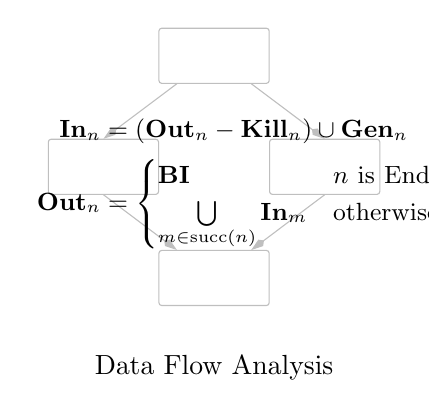
\begin{tikzpicture}[r/.style={rectangle,draw,minimum width=2cm,minimum height=1cm,rounded corners=1pt},baseline={([yshift=-.5ex]current bounding box.center)},line cap=round]
   \tikzset{@/.style={opacity=1}}
   \def\scaler{1}
   \only<7->{\def\scaler{0.5}\tikzset{@/.style={opacity=.5,scale=.5,every node/.style={transform shape}}}}
   \scope[@]
   \scope[black!25!white,scale=.7,every node/.style={transform shape}]
   \node[r] (@) at(0,0) {};
   \node[r, below left=1cm] (@a) at(@.south) {};
   \node[r, below right=1cm] (@b) at(@.south) {};
   \node[r,below=1cm] (@c) at(current bounding box.south) {};
   \draw[-Kite] (@) -- (@a.north);
   \draw[-Kite] (@) -- (@b.north);
   \draw[-Kite] (@a.south) -- (@c);
   \draw[-Kite] (@b.south) -- (@c);
   \endscope
   \node[align=center,text width=4.5cm] at(current bounding box.center) {\small%
\begin{align*}
   \mathbf{In}_n &= (\mathbf{Out}_n - \mathbf{Kill}_n) \cup \mathbf{Gen}_n \\
   \mathbf{Out}_n &= \begin{cases}
      \mathbf{BI} & n \text{~is End} \\
      \bigcup\limits_{m \in \text{succ}(n)} \mathbf{In}_m & \text{otherwise}
   \end{cases}
\end{align*}
   };
   \onslide<6->{
      \node[below=5mm] at(current bounding box.south) {Data Flow Analysis};
   }
   \endscope
\end{tikzpicture}
\end{uncoverenv}
\hspace*{4.5em}\onslide<8->{\large\ldots}
\end{uncoverenv}
\end{frame}

\newsavebox\CodeFile
\begin{lrbox}{\CodeFile}
\scalebox{1.45}{%

\begin{tikzpicture}
   \draw[rounded corners=1.5pt,fill=white] (0,0) |- ++(.6,-.8) [sharp corners] -- ++(0,.6) -- ++(-.2,.2) coordinate (@rl) [rounded corners=2pt] -- cycle (@rl) |- ++(.2,-.2);
   \draw[thick,line cap=round,lightgray] (.1,-.1) -- ++(.2,0)
      % for what have I written random code generation? :C 
      (.1,-.15) -- ++(.1,0) ++(.05,0) -- ++(.1,0)
      (.125,-.2) -- ++(.15,0)++(.05,0)--++(.025,0)
      (.1,-.25) -- ++(.3,0)
      (.125,-.3) --++(.2,0)++(.05,0)--++(.05,0)
      (.125,-.35) --++(.15,0)++(.05,0)--++(.1,0)
      (.15,-.4)--++(.2,0)
      (.15,-.4)--++(.1,0)++(.05,0)--++(.05,0)
      (.125,-.45)--++(.05,0)
      (.1,-.5)--++(.066,0)++(.05,0)--++(.15,0)
      (.1,-.6)--++(.15,0)++(.05,0)--++(.15,0)
      (.1,-.65)--++(.2,0)
      (.1,-.7)--++(.1,0)++(.05,0)--++(.15,0)
   ;
\end{tikzpicture}}
\end{lrbox}
\newsavebox\MagicPenguin
\savebox\MagicPenguin{\tikz{\pingu[witch hat,eyes wink,wings wave,bee,blush,santa beard]}}
\newsavebox\MagicPenguinTwo
\savebox\MagicPenguinTwo{\tikz{\pingu[witch hat,eyes shiny,bee,santa beard]}}
\begin{frame}{What we want\ldots}
   \frametitle<1>{\strut What we want\ldots~}%
   \frametitle<2->{\strut\textcolor{gray}{What we want\ldots~}Tools}%
   \centering\kern1.345em
   \begin{uncoverenv}<3->
   \begin{tikzpicture}[o/.style={outer sep=0pt,inner sep=0pt},line cap=round,Rect/.style={draw,rectangle,rounded corners=3pt,inner sep=4pt,outer sep=1mm},draw=gray,every path/.append style={thick}]
      \node[o] (@) at (0,0) {\usebox\CodeFile};
      \pgfonlayer{background}
      \scope[transparency group,opacity=.4]
      \node[o,rotate around={-30:(@.south east)},anchor=south east] at(@.south east) {\usebox\CodeFile};
      \node[o,rotate around={-12:(@.south east)},anchor=south east] at(@.south east) {\usebox\CodeFile};
      \endscope
      \endpgfonlayer
      \node[below] at(@.south) {\small Project};
      \onslide<3->{
         \node[right=1.33cm,Rect,minimum width=4.5em] (@magic) at(@.east) {~\vphantom{Magic}{\only<8->{\only<9->{\color{gray!34}}\clap{Magic}}}\only<9->{\clap{\kern-.8pt\textbf{Tools}}}~\null};
         \draw[-Kite] ([xshift=5mm]@.east) -- (@magic.west);
      }
      % and how can we achieve that?... magic :sparkles: but as there is no magic, we need tools... and algorithms
      \onslide<8->{
         \node[above right,xshift=1.3mm] at(@magic.north west) {\scalebox{.45}{\only<-8|handout:0>{\kern-8.5pt\usebox\MagicPenguin}\only<9->{\usebox\MagicPenguinTwo}}};
      }
      \coordinate (@) at(@magic.east);
      \foreach[count=\i] \usecase/\targeti in {Security/4, Maintenance/5, Comprehension/6, Optimization/7, Usability/7, \ldots/7} {
      \pgfmathsetmacro\rot{-11*\i+38.75}
         \onslide<\targeti->{
            \node[right=1cm,Rect,rotate around={\rot:([xshift=-9mm]@.east)},minimum width=8em,fill=white] (@uc-\i) at (@.east) {\strut\usecase};
            \draw[-Kite,sharp corners] (@.east) -- ++(4.2mm,0) [rounded corners=1pt] arc (0:\rot:9mm) -- (@uc-\i.west);
         }
      }
      \onslide<11->{
         \scope[gray]
         \node[right] at (@uc-1.east) {\small injections, leaks,~\ldots};
         \node[right] at (@uc-2.east) {\small code clones, deprecation,~\ldots};
         \node[right] at (@uc-3.east) {\small documentation, structure,~\ldots};
         \node[right] at (@uc-4.east) {\small better algorithms, memoization,~\ldots};
         \node[right] at (@uc-5.east) {\small color deficiency, size,~\ldots};
         \node[right] at (@uc-6.east) {\small \only<-11|handout:0>{\ldots}\only<12->{architecture recovery, refactoring,~\ldots}};
         \endscope
      }
      \onslide<13->{
         \draw[Kite-] (@magic.south) -- ++(0,-.66) node[below,align=center,font=\footnotesize] {SonarQube\rlap{\textsuperscript{1}}, Teamscale\rlap{\textsuperscript{2}},\\lintr\rlap{\textsuperscript{3}}, CodeQL\rlap{\textsuperscript{4}}, \ldots};
      }
   \end{tikzpicture}

   \begin{tikzpicture}[overlay,remember picture]
      \onslide<10->{%
         \node[above=9mm,lightgray] at(current page.south) {\footnotesize\enquote{Any sufficiently advanced technology is indistinguishable from magic.} --- Arthur C. Clarke};% 3rd law
      }
      \onslide<13->{\node[bottom note,above right,yshift=5mm] at(current page.south west) {%
         \textsuperscript{1}\,\href{https://www.sonarsource.com/}{sonarsource.com}, \textsuperscript{2}\,\href{https://teamscale.com/}{teamscale.com}, \textsuperscript{3}\,\href{https://lintr.r-lib.org/}{lintr.r-lib.org}, \textsuperscript{4}\,\href{https://codeql.github.com/}{codeql.github.com}%
      };}
   \end{tikzpicture}
   % TODO: tool examples
   % rather list concrete problems than tools
\end{uncoverenv}
\end{frame}

\usetikzlibrary{backgrounds,graphs,arrows.meta,decorations.pathreplacing}

\definecolor{BaseGray}{RGB}{66,66,66} % rgb(66,66,66)

\colorlet{SoftGray}{BaseGray!40}
\colorlet{BackGray}{BaseGray!5}
\colorlet{SoftTextGray}{BackGray!60!SoftGray}


\tikzset{
   FunctionDef/.style={
      draw=BaseGray,
      fill=BaseGray,
      minimum width=1.55cm,
      minimum height=1cm,
      text=white,
      font=\bfseries,
      text centered,
      inner sep=0pt,
      rounded corners=1mm,
      outer sep=2pt
   },
   Blob/.style={
      draw=SoftGray,
      fill=SoftGray,
      minimum size=4mm,
      text=white,
      circle,
      font=\bfseries,
      text centered,
      inner sep=0pt,
      outer sep=2pt
   },
   Def/.style={
      Blob,
      rectangle, rounded corners=1mm
   },
   ActiveBlob/.style={
      Blob,
      draw=BaseGray!80!white, fill=BaseGray!80!white
   },
   FunctionBack/.style={
      fill=BackGray,
      % draw=SoftGray,
      rounded corners=2mm,
      rectangle
   },
   Link/.style={
      draw=SoftGray,
      line width=1.5pt,
      line cap=round,
      line join=round,
      -%
   },
   FuncLink/.style={
      Link,
      draw=SoftGray,
      dotted
   },
   Cursor/.style={
      fill=BackGray,
      draw=BaseGray,
      line join=round,
      line cap=round
   },
   Hover-Over/.style={
      fill=BackGray,
      draw=SoftGray,
      opacity=.5,
      draw opacity=1,
      rounded corners=1mm,
      line join=round,
      line cap=round
   },
   Line-Of-Text/.style={
      fill=#1,
      draw=none,
      rounded corners=1.5pt,
      inner sep=1pt,
      minimum width=1cm,
      minimum height=6.5pt
   },
   Input-Base/.style={
      fill=BackGray,
      draw=SoftGray,
      rounded corners=1mm,
      inner sep=1pt,
      minimum width=2cm,
      minimum height=12pt
   },
   % code sub-styles
   A/.style={Line-Of-Text=SoftTextGray},
   B/.style={},
   C/.style={Line-Of-Text=SoftGray},
   path image shift/.style={},
   path image/.style 2 args={path picture={\node at ([path image shift]path picture bounding box.center) {\includegraphics[width=#2]{#1}};}},
}


\newcommand\Back[4][]{
   \pgfonlayer{background}
   \fill[FunctionBack,#1] ([xshift=-2mm,yshift=-2mm]#2.south west) rectangle ([xshift=2mm,yshift=2mm]#3.north east);
   \coordinate (#4@north) at([yshift=2mm]0,0|-#3.north);
   \coordinate (#4@west) at([xshift=-2.5mm]0,0-|#2.west);
\endpgfonlayer
}
\newsavebox\UiBox
\begin{lrbox}{\UiBox}
\begin{tikzpicture}
   \node[FunctionDef] (F) at (0,0) {};

   \scope[shift={(F.south)},yshift=-1.5cm]
      \node[Def] (a1) at (-1,0) {};
      \node[Blob] (b1) at (.5,-.25) {};
      \node[ActiveBlob] (c1) at (1.55,-1.35) {};
      \node[Blob] (d1) at (-0.5,-1.6) {};
      \node[Blob] (e1) at (1.8,.25) {};
      \node[Blob] (f1) at (-2.2,-1.5) {};

      \graph[edges={Link}] {
         (a1) -> { (b1), (c1) } -> (d1) -> (e1) -> (a1),
         (f1) -> { (a1), (d1) }
      };

      \Back{f1}{e1}{f1}

      \draw[FuncLink] (f1@north) -- (F.south);
   \endscope

   \node[Blob] (a) at (2.5,0) {};
   \node[Blob] (b) at (1.5,1) {};
   \node[Blob] (c) at (3,2) {};
   \node[Blob] (d) at (-2.5,0.5) {};
   \node[Def] (e) at (-2.5,1.5) {};
   \node[Blob] (f) at (-3,2.5) {};
   \node[Blob] (g) at (-3.5,-1) {};
   \node[Blob] (h) at (-3,-2.5) {};

   \node[FunctionDef] (F2) at(5,-.5) {};
   \node[Blob] (u) at(5.5,1) {};

   \scope[shift={(F2.east)},xshift=1.5cm]

      \node[Blob] (a2) at (0,1.15) {};
      \node[Def] (b2) at (.75,1.85) {};
      \node[Blob] (c2) at (-.5,-.85) {};

      \node[Blob] (d2) at (1.33,0.25) {};
      \node[FunctionDef] (e2) at (2,-.75) {};

      \node[Blob] (f2) at (3.75,1.5) {};
      \node[Blob] (g2) at (2.75,2.5) {};

      \scope[shift=(e2.south), yshift=-1cm]
         \node[ActiveBlob] (a3) at (-1,0) {};
         \node[Blob] (b3) at (1,0) {};
         \draw[Link] (a3) -- (b3);
         \Back[white]{a3}{b3}{a3} % for coordinate
      \endscope

      \coordinate (ll) at ([yshift=-2mm]a3.south west-|c2.west);
      \coordinate (ur) at (f2.north east|-g2.north);

      \Back{ll}{ur}{e2}
      \draw[FuncLink] (e2@west) -- (F2.east);

      % draw inner later
      \Back[white]{a3}{b3}{xx} % for the overlay :D
      \draw[FuncLink] (a3@north) -- (e2.south);

      \graph[edges={Link}] {
         (a2) -> (b2) -> { (c2) , (d2) },
         (d2) -> { (e2), (f2) },
         (f2) -> (g2),
         (c2) -> (a3)
      };
   \endscope

   \graph[edges={Link}] {
      (F) -> { (a), (b) },
      (a) -> (e1),
      (b) -> (c) -> (b2),
      (b) -> (d) -> { (F), (e) },
      (e) -> (f) -> (c),
      (d) -> (g) -> (h) -> (f1),
      (u) -> (F2)
   };

   \coordinate (cursor-pos) at ([xshift=-1.65mm,yshift=2mm]F2.south east);
   \draw[Cursor,rotate around={28:(cursor-pos)}]  [rounded corners=2.25pt] (cursor-pos)  [rounded corners=2.25pt] -- ++(4pt,-9.5pt) [rounded corners=2pt] -- ++(-4pt,3pt) [rounded corners=2.25pt]-- ++(-4pt,-3pt) -- cycle;
   \node[below left,xshift=-1mm,yshift=1.15mm,Hover-Over,minimum width=1.25cm,minimum height=6mm] (hoverover) at(cursor-pos) {%
      %
   };
   % \scope[opacity=.95,transparency group]
      \fill[Line-Of-Text=SoftGray] ([shift={(2pt,-2pt)}]hoverover.north west) rectangle ++(7.5mm,-4pt);
      \fill[Line-Of-Text=SoftTextGray] ([shift={(2pt,-7.5pt)}]hoverover.north west) rectangle ++(11mm,-3pt);
      \fill[Line-Of-Text=SoftTextGray] ([shift={(2pt,-7.5pt-4.5pt)}]hoverover.north west) rectangle ++(8mm,-3pt);
   % \endscope

   % TODO: outsource window?
   \coordinate (wul) at ([shift={(-5mm,6mm)}]current bounding box.north west);
   \coordinate (wur) at ([shift={(5mm,6mm)}]current bounding box.north east);
   \draw[thin,rounded corners=3pt,SoftGray] ([shift={(-5mm,-5mm)}]current bounding box.south west) rectangle (wur);
   % just "overlay" the top :D
   \filldraw[SoftGray] ([yshift=-1mm]wul) coordinate (@) -- (wur|-@) [rounded corners] |- ([yshift=2.5mm]wul) [sharp corners] -- cycle;

   \fill[Line-Of-Text=BackGray] ([yshift=1.35mm,xshift=4pt]wul) rectangle ++(2cm,-1.27mm);
   \node[above left,BackGray] at([yshift=-1.33mm,xshift=-1mm]wur) {\smash{\scalebox{.9}{\scriptsize\faAngleDown~~\faAngleUp~~\faTimesCircle}}};

   \coordinate (root control window) at(current bounding box.south west);

   \scope[shift={(current bounding box.south east)},shift={(-7cm,4.5mm)}]
      \coordinate (wul) at (0,0);
      \coordinate (wur) at (8.5,0);

      \draw[thin,rounded corners=3pt,SoftGray,fill=white] (0,-5) rectangle (wur);

      % code line
      \draw[thin,BackGray] ([xshift=1cm,yshift=-1mm]wul) coordinate (@) -- (@|-0,-5);
      % line numbers and code
      \foreach[count=\i from 0] \Code in {
         {1/A,0.5/A,5/C,2/A},
         {1.5/B,3/A,0.5/A,2/A},
         {},
         {1.5/B,0.5/A,3/A},
         {1/A},
         {},
         {5/A,0.5/A,2/A},%
         {0.5/A,5/A,3/A,0.5/A,2/A,5.5/A},
         {},
         {1/C,0.5/A,1/A,0.5/A,1/A,0.5/A,0.15/B,0.5/A},
         {1.5/B,3/A,0.5/A,1/C,2/A,1.5/A,1/C,1.5/A},
         {1.5/B,0.75/A,0.5/A,1.5/A,0.5/A,1/A},
         {1.5/B,3/A,0.5/A,2/A},
         {1.5/B,2/A,0.5/A,2/A},
         {1/A}%
      } {
         \ifnum\i<6 \def\Width{4mm} \else \def\Width{6mm} \fi
         \fill[Line-Of-Text=BackGray] ([yshift=-1mm,xshift=8mm]wul|-0,-\i*0.33*10mm+1mm) rectangle ++(-\Width,-2mm);
         \def\XShift{5}
         \foreach \CW/\Style in \Code {
            \ifstrequal{\Style}{B}{\def\RandomSuffix{0}}{\def\RandomSuffix{(rand*0.4mm+0.75mm)}}
            \pgfmathsetmacro\w{3*\CW mm+\RandomSuffix}
            \path[\Style] ([yshift=-1mm,xshift=1cm+\XShift pt]wul|-0,-\i*0.33*10mm+1mm) rectangle ++(\w pt,-2mm);

            \pgfmathsetmacro{\XShift}{\XShift+\w pt+1.5mm}
            \xdef\XShift{\XShift}
         }
      }

      % slider
      \draw[Line-Of-Text=SoftTextGray,rounded corners=.325mm] ([yshift=-4cm+5mm,xshift=-1mm]wur) rectangle ++(-.75mm,-1cm);

      % just redraw the frame :D
      \draw[thin,rounded corners=3pt,SoftGray] (0,-5) rectangle (wur);

      \filldraw[SoftGray] ([yshift=-1mm]wul) coordinate (@) -- (wur|-@) [rounded corners] |- ([yshift=2.5mm]wul) [sharp corners] -- cycle;

      \fill[Line-Of-Text=BackGray] ([yshift=1.35mm,xshift=4pt]wul) rectangle ++(1.66cm,-1.27mm);
      \node[above left,BackGray] at([yshift=-1.33mm,xshift=-1mm]wur) {\smash{\scalebox{.9}{\scriptsize\faAngleDown~~\faAngleUp~~\faTimesCircle}}};

   \endscope

   % window for controls
   \scope[shift={(root control window)},shift={(-1cm,-5mm)}]
      \draw[thin,rounded corners=3pt,SoftGray,fill=white] (0,-4) rectangle ++(8.33cm,4cm);
      \coordinate (wul) at (0,0);
      \coordinate (wur) at (8.33,0);

      \node[Input-Base,minimum width=6cm,below right=3mm] (slice-criterion-input) at (wul) {};
      \fill[Line-Of-Text=SoftTextGray] ([yshift=1mm,xshift=4pt]slice-criterion-input.west) rectangle ++(1.25cm,-2mm);
      \fill[Line-Of-Text=SoftTextGray] ([yshift=1mm,xshift=4pt+1.25cm+2mm]slice-criterion-input.west) rectangle ++(1cm,-2mm);

      % frame stuff
      \filldraw[SoftGray] ([yshift=-1mm]wul) coordinate (@) -- (wur|-@) [rounded corners] |- ([yshift=2.5mm]wul) [sharp corners] -- cycle;
      \node[right=1mm,SoftGray,] at(slice-criterion-input.east) {\tiny\faChevronRight~~~~~\faPieChart~~\faUpload~~\faDownload};

      % logging window
      \draw[rounded corners=3pt,BackGray,fill=white] ([xshift=3mm,yshift=-1cm]wul) rectangle ([xshift=-3mm,yshift=-3.7cm]wur);

      % log
      \foreach[count=\i from 0] \Code in {
         {1/A,2/A,6/A,1/B,3/A},
         {1.5/B,3/A,2/A,2/A,1/A},
         {1.5/B,2/A,3/A,1/A,2/A,3/A,1/A},
         {1.5/B,4/A,1/A},
         {1.5/B,3/A,2/A,2/A,1/A},
         {1.5/B,3/A,1/A,4/A,1/A},
         {},
         {1/A,2/A,6/A},
         {1/A,2/A,3/A,1.5/A,2.5/A},
      } {
         \def\XShift{5}
         \foreach \CW/\Style in \Code {
            \ifstrequal{\Style}{B}{\def\RandomSuffix{0}}{\def\RandomSuffix{(rand*0.4mm+0.75mm)}}
            \pgfmathsetmacro\w{3*\CW mm+\RandomSuffix}
            \path[\Style] ([yshift=-2.5mm-1cm,xshift=3.25mm+\XShift pt]wul|-0,-\i*0.28*10mm+1mm) rectangle ++(\w pt,-1.75mm);

            \pgfmathsetmacro{\XShift}{\XShift+\w pt+1mm}
            \xdef\XShift{\XShift}
         }
      }

      % slider
      \draw[Line-Of-Text=SoftTextGray,rounded corners=.325mm] ([yshift=-2cm+3mm,xshift=-4mm]wur) rectangle ++(-.75mm,-1cm);

      % head
      \fill[Line-Of-Text=BackGray] ([yshift=1.35mm,xshift=4pt]wul) rectangle ++(5mm,-1.27mm);
      \fill[Line-Of-Text=BackGray] ([yshift=1.35mm,xshift=4pt+6.5mm]wul) rectangle ++(1cm,-1.27mm);
      \node[above left,BackGray] at([yshift=-1.33mm,xshift=-1mm]wur) {\smash{\scalebox{.9}{\scriptsize\faAngleDown~~\faAngleUp~~\faTimesCircle}}};
   \endscope
\end{tikzpicture}
\end{lrbox}


\begin{frame}{\strut What do they\ldots~do?}
% they take input, textual, syntactical, semantic (call graphs, pdg, ...), metadata, historical information, requirements, annotations (types, contracts), ...
\hspace*{-3.5mm}
\begin{tikzpicture}[o/.style={outer sep=0pt,inner sep=0pt}]
   \onslide<2->{%
      \node[o] (@) at (0,0) {\usebox\CodeFile};
      \node[above=2.5mm,xshift=1.15mm,gray] at(@.north) {\tiny They take \textbf{\normalsize Input}};
   }
   \pgfonlayer{background}
   \onslide<2->{%
   \scope[transparency group,opacity=.4]
   \node[o,rotate around={-30:(@.south east)},anchor=south east] at(@.south east) {\usebox\CodeFile};
   \node[o,rotate around={-12:(@.south east)},anchor=south east] at(@.south east) {\usebox\CodeFile};
   \endscope}
   \endpgfonlayer
   \begin{uncoverenv}<3->
   \coordinate (@) at(@.east);
   \foreach[count=\i] \usecase/\targeti in {{\raisebox{1pt}{Textual}}/4,Syntactical/5, Semantical/6, Historical/7, Annotated/8, {\only<-9|handout:0>{\ldots}\only<10->{\raisebox{-3pt}{Metadata,~\ldots}}}/9} { % program spectra, hardware, contexts, ...
   \pgfmathsetmacro\rot{-24*\i+66}
      \onslide<\targeti->{
         \path ([xshift=.5mm]@.east)++(\rot+10:1mm) coordinate (@a);
         \fill[opacity=.18,gray] (@a.east) -- ++(\rot:1.5cm) arc (\rot:\rot+20:1.5cm) -- cycle;
         \draw[thick,gray] (@a.east)++(\rot:1.5cm) arc (\rot:\rot+20:1.5cm);
         \path (@a.east) -- ++(1.05*\rot+10:1.6cm) node[right,font=\small,darkgray] (@uc-\i) {\vphantom{a}\smash{\usecase}};
      }
   }
   \node[above=1.65mm,xshift=1mm,gray] at(current bounding box.north) {\tiny And use \textbf{\normalsize Perspectives} \rlap{(often combined)}};
   \end{uncoverenv}
   \onslide<11->{%
      \draw[Kite-,gray] ([xshift=6.25mm,yshift=-1mm]current bounding box.south) to[out=-90,in=0] ++(-4.5mm,-5mm) node[below left,yshift=.42\baselineskip,align=right,text width=2.5cm,font=\tiny] {Some of those are the result of other static or dynamic analyses};
   }
   \begin{uncoverenv}<12->
      \node[right,yshift=-2mm,xshift=1cm,align=left,font=\small,darkgray,text width=3.25cm] (@techn) at(current bounding box.east){{\onslide<13->{\subnode{tc-search}{Text/Code Search}\strut}}~\\[4mm]\strut{\onslide<14->{\subnode{clustering}{Clustering}}}~\\[4mm]\strut{\onslide<15->{\subnode{ai}{Abstract Domains}}}~\\[4mm]\strut{\onslide<16->{\subnode{df-constraints}{Dataflow Constraints}}}~\\[1mm]\strut{\onslide<16->{\centerline{\footnotesize\(\vdots\)}}}};
      \onslide<12->{
         \node[above=2.5mm,gray,xshift=-4.5mm] at(@techn.north) {\tiny To apply \textbf{\normalsize Theory}};
      }
   \end{uncoverenv}
   \scope[gray,line cap=round]
   \only<17->{
      \draw ([yshift=1.5pt]@uc-1.east) -- ([yshift=-2.5mm]@techn.north west);
      \draw ([yshift=1.5pt]@uc-2.east) -- ([yshift=-2.5mm]@techn.north west);
      \draw[densely dotted] ([yshift=1.5pt]@uc-3.east) -- ([yshift=-2.5mm]@techn.north west);
   }
   \only<18->{
      \draw ([yshift=1.5pt]@uc-1.east) -- ([yshift=-10.5mm]@techn.north west);
      \draw ([yshift=0pt]@uc-2.east) -- ([yshift=-10.5mm]@techn.north west);
      \draw ([yshift=1.5pt]@uc-4.east) -- ([yshift=-10.5mm]@techn.north west);
      
      \draw ([yshift=-1pt]@uc-2.east) -- ([yshift=-18.5mm]@techn.north west);
      \draw ([yshift=-1pt]@uc-3.east) -- ([yshift=-18.5mm]@techn.north west);
      \draw ([yshift=1.5pt]@uc-5.east) -- ([yshift=-18.5mm]@techn.north west);
      
      \draw ([yshift=-1pt]@uc-2.east) -- ([yshift=-26mm]@techn.north west);
      \draw ([yshift=-1pt]@uc-3.east) -- ([yshift=-26mm]@techn.north west);
   }
   \endscope
   \begin{uncoverenv}<19->
      
      \onslide<20->{\node[right=7.5mm] (@) at(current bounding box.east) {\resizebox*!{2.85cm}{\usebox\UiBox}};
      \scope[transparency group,opacity=.5,every path/.append style={line cap=round,line width=.5pt}]
         \draw[-Kite,gray] ([yshift=-2.5mm,xshift=-6.5mm]@techn.north east) to[out=0,in=180] ([xshift=1.5mm,yshift=-6.35mm]@.west);
         \draw[-Kite,gray] ([yshift=-10.5mm,xshift=-18.5mm]@techn.north east) to[out=0,in=180] ([xshift=7.15mm,yshift=-1.35mm]@.west);
         \draw[-Kite,gray] ([yshift=-18.5mm,xshift=-6.25mm]@techn.north east) to[out=0,in=180] ([xshift=26.15mm,yshift=-9.35mm]@.west);
         \draw[-Kite,gray] ([yshift=-26mm,xshift=-2.5mm]@techn.north east) to[out=0,in=180] ([xshift=26.15mm,yshift=-9.35mm]@.west);
      \endscope
      }
      \node[above, gray] at(@.north) {\tiny And \textbf{\normalsize Communicate} or \textbf{\normalsize Use} results};
   \end{uncoverenv}
\end{tikzpicture}
\end{frame}


% #1 url #2 name
\def\Logo#1#2{\href{#1}{\includegraphics[height=3cm,width=3cm,keepaspectratio]{logos/#2.png}}}

\begin{frame}{Let's Look at Tools}
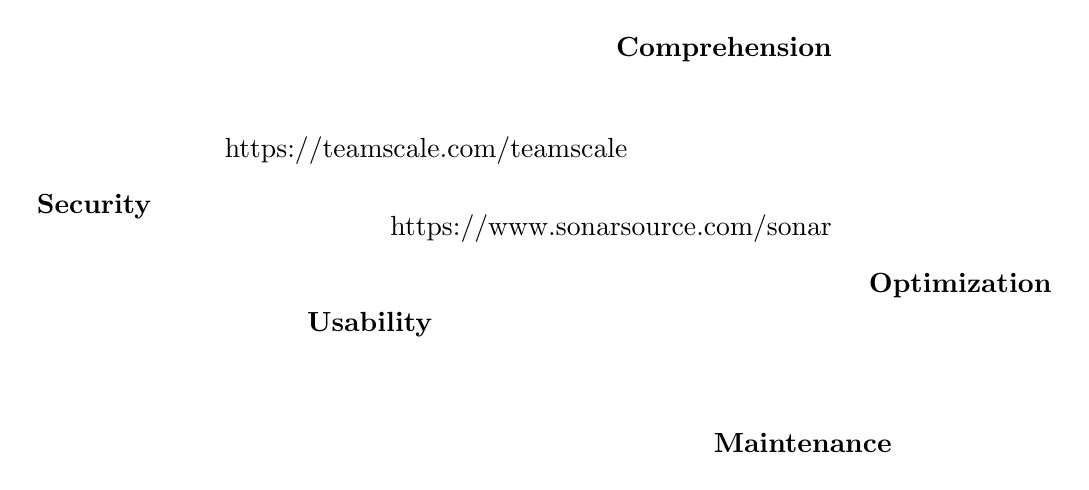
\begin{tikzpicture}
   \tikzset{@/.style={}}
   \only<2->{\tikzset{@/.style={opacity=.2}}}
   \node[@] (sec) at (-2,0) {\bfseries Security};
   \node[@] (mai) at (7,-3) {\bfseries Maintenance};
   \node[@] (com) at (6,2) {\bfseries Comprehension};
   \node[@] (opt) at (9,-1) {\bfseries Optimization};
   \node[@] (sec) at (1.5,-1.5) {\bfseries Usability};
   % TODO: block of compilers; language servers
   \onslide<3->{
      \node[xshift=8.5mm,yshift=2mm] (sonar) at (current bounding box.center) {\Logo{https://www.sonarsource.com/}{sonar}};
   }
   \onslide<4->{
      \node[xshift=-15mm,yshift=12mm] (sonar) at (current bounding box.center) {\Logo{https://teamscale.com/}{teamscale}};
   }
\end{tikzpicture}
   
\end{frame}

\begin{frame}
   Wir hatten Abstraktionen, Theorie, jetzt mal mehr wie das abläuft
   ~> Programm rein, CFG, Basic Blocks, AST, analysis passes, completeness vs. soundness
\end{frame}

\begin{frame}
   Tabelle mit astree, sonar lint cube, lintr, .. aber eben auch nicht fehlerfinden sondern z.b. globals, renaming, etc.
\end{frame}

\begin{frame}
   TODO: dynamic analysis alternative
\end{frame}

% \section{The Why}
% \subsection[Motivation]{Initial Motivation}
% \begin{frame}[fragile,label=main-example]{\insertsection}
% x
% \end{frame}

\renewcommand*{\bibfont}{\tiny}

\AtBeginSection{}
\begin{frame}[allowframebreaks]{References}
   \printbibliography[title={}] % TODO
\end{frame}

\end{document}